% eilmer.tex

\section{Gas Dynamics}
\label{sec:gas-dynamics}  % actually, it should be mbcns2...
%
The code is formulated around the integral form of the Navier-Stokes equations, which can be expressed as
\begin{equation}
 \frac{\partial}{\partial t} \int_{V} U dV = - \oint_{S} \left ( \overline{F}_{i} - \overline{F}_{v} \right ) \cdot \hat{n}~dA + \int_{V} Q dV \text{ , }
 \label{eq:NS}
\end{equation}
where $S$ is the bounding surface and $\hat{n}$ is the outward-facing unit normal of the control surface.
Two-dimensional and three-dimensional formulations are implemented somewhat separately in \texttt{Eilmer3},
however, there is much of the formulation and code that is the same for both cases. 

\subsection{Governing Equations for Axisymmetric, Two-Dimensional Flow}
%
For axisymmetric flow, the symbol $V$ in Eq.(\ref{eq:NS}) is the volume 
and $A$ the area of the cell boundary per unit radian in the circumferential direction.
The array of conserved quantities is dependent on the thermal model under consideration, 
and for the thermal nonequilibrium models is
\begin{equation}
 U = \left [ \begin{array}{c} 
                 \rho \\
                 \rho u_{x} \\
                 \rho u_{y} \\
                 \rho E \\
                 \rho e_{v_{m}} \\
                 \rho e_{e} \\
                 \rho f_{s}
              \end{array} \right ] \text{ . }
 \label{eq:U_vector}
\end{equation}
Here, the conserved quantities are respectively density, $x$-momentum per volume, $y$-momentum per volume, 
total energy per volume, vibrational energy for mode $m$, electronic-electron energy and mass density of species $s$.
Note that $\rho e_{e}$ includes both bound and free electron energy.
We choose to solve both total and all individual species continuity equations to add rigour to our solver: the redundant information gives us a good idea when the
numerics are running into trouble.  Conversely, when only solving $n-1$ species equations, it is easier for undetected error in mass fractions to accumulate.
Thus for 11 species air with 6 vibrating molecules and the inclusion of electrons, 
for example, there are 22 conserved quantities.  

\medskip
The flux vectors are divided into inviscid and viscous contributions.  
The inviscid component in thermal nonequilibrium is
\begin{equation}
 \overline{F}_{i} = \left [ \begin{array}{c}
                               \rho u_{x} \\
                               \rho u_{x}^{2} + p \\
                               \rho u_{y} u_{x} \\
                               \rho E u_{x} + p u_{x} \\
                               \rho e_{v_{m}} u_{x} \\
                               \rho e_{e} u_{x} + p_{e} u_{x} \\
                               \rho f_{s} u_{x}
                            \end{array} \right ] \hat{i} 
                  + \left [ \begin{array}{c} 
                               \rho u_{y} \\
                               \rho u_{x} u_{y} \\
                               \rho u_{y}^{2} + p \\
                               \rho E u_{y} + p u_{y} \\
                               \rho e_{v_{m}} u_{y} \\
                               \rho e_{e} u_{y} + p_{e} u_{y} \\
                               \rho f_{s} u_{y}
                            \end{array} \right ] \hat{j} \text{ , }
 \label{eq:F_i}
\end{equation}
and the viscous component is
\begin{equation}
 \overline{F}_{v} = \left [ \begin{array}{c} 
                                0 \\
                                \tau_{xx} \\
                                \tau_{yx} \\
                                \tau_{xx} u_{x} + \tau_{yx} u_{y} + q_{x} \\
                                q_{x,v_{m}} \\
                                q_{x,e} \\
                                J_{x,s}
                            \end{array} \right ] \hat{i} 
                   + \left [ \begin{array}{c}
                                 0 \\
                                 \tau_{xy} \\
                                 \tau_{yy} \\
                                 \tau_{xy} u_{x} + \tau_{yy} u_{y} + q_{y} \\
                                 q_{y,v_{m}} \\
                                 q_{y,e} \\
                                 J_{y,s}
                             \end{array} \right ] \hat{j} \text{ . }
 \label{eq:F_v}
\end{equation}
where the axisymmetric viscous stresses are
\begin{eqnarray}
 \tau_{xx} &=& 2 \mu \frac{\partial u_{x} }{\partial x} 
               + \lambda \left ( \frac{\partial u_{x}}{\partial x} 
                                 + \frac{\partial u_{y}}{\partial y} 
                                 + \frac{u_{y}}{y} \right ) \text{ , } \nonumber \\
 \tau_{yy} &=& 2 \mu \frac{\partial u_{y} }{\partial y} 
               + \lambda \left ( \frac{\partial u_{x}}{\partial x} 
                                 + \frac{\partial u_{y}}{\partial y} 
                                 + \frac{u_{y}}{y} \right ) \text{ , } \nonumber \\
 \tau_{xy} = \tau_{yx} &=& \mu \left ( \frac{\partial u_{x}}{dy} 
                                     + \frac{\partial u_{y}}{dx} \right ) \text{ , }
 \label{eq:taus}
\end{eqnarray}
and where the secondary viscosity coefficient $\lambda$ is expressed 
in terms of the primary coefficient $\mu$ via Stokes hypothesis, $\lambda = - \frac{2}{3} \mu$. 
The viscous heat fluxes are
\begin{eqnarray}
 q_{x} &=& k_{tr} \frac{\partial T}{\partial x} + \sum_{s=\text{mol.}} k_{v_{s}} \frac{\partial T_{v_{s}}}{\partial x} + k_{e} \frac{\partial T_{e}}{\partial x} + \sum_{s=\text{all}}{ J_{x,s} h_{s} } \text{ , } \nonumber \\
 q_{y} &=& k_{tr} \frac{\partial T}{\partial y} + \sum_{s=\text{mol.}} k_{v_{s}} \frac{\partial T_{v_{s}}}{\partial y} + k_{e} \frac{\partial T_{e}}{\partial y} + \sum_{s=\text{all}}{ J_{y,s} h_{s} } \text{ , } \nonumber \\
 q_{x,v_{m}} &=& k_{v_{m}} \frac{\partial T_{v_{m}}}{\partial x} + J_{x,m} h_{v_{m}} \text{ , } \nonumber \\
 q_{y,v_{m}} &=& k_{v_{m}} \frac{\partial T_{v_{m}}}{\partial y} + J_{y,m} h_{v_{m}} \text{ , } \nonumber \\
 q_{x,e} &=& k_{e} \frac{\partial T_{e}}{\partial x} + \sum_{s=\text{all}}{ J_{x,s} h_{e_{s}} } \text{ , } \nonumber \\
 q_{y,e} &=& k_{e} \frac{\partial T_{e}}{\partial y} + \sum_{s=\text{all}}{ J_{y,s} h_{e_{s}} } \text{ . } \label {eq:qs}
\end{eqnarray}

\medskip
The vector of source terms is separated into geometric, chemistry, thermal energy exchange and radiation contributions 
in order to apply the operator-splitting integration approach, Eq.~\ref{eq:Q_sum}.
\begin{equation}
 Q = Q_{\text{geom.}} + Q_{\text{chem.}} + Q_{\text{therm.}} + Q_{\text{rad.}}
 \label{eq:Q_sum}
\end{equation}
The geometric source term vector for axisymmetric geometries is
\begin{equation}
 Q_{\text{geom.}} = \left [ \begin{array}{c} 0 \\ 0 \\ \left ( p - \tau_{\theta \theta} \right ) A_{xy} / V \\ 0 \\ 0 \\ 0 \end{array} \right ] \text{ , }
 \label{eq:Q_geom}
\end{equation}
where $A_{xy}$ is the projected area of the cell in the (x,y)-plane and 
\begin{equation}
 \tau_{\theta\theta} = 2 \mu \frac{u_{y}}{y} + \lambda \left ( \frac{\partial u_{x} }{\partial x} + \frac{\partial u_{y} }{\partial y} + \frac{u_{y}}{y} \right ) \text{ . }
 \label{eq:tau00}
\end{equation}
For planar geometries $Q_{\text{geom.}}$ is a zero vector.
See the original ICASE report \cite{jacobs_91d} for a derivation of these terms.

\medskip
The chemistry source term vector is
\begin{equation}
 Q_{\text{chem.}} = \left [ \begin{array}{c} 0 \\ 0 \\ 0 \\ 0 \\ \Omega^{VC}_{m} \\ \sum_{s=\text{ion.}} \Omega^{EC}_{s} \\ \dot{\omega_{s}} \end{array} \right ] \text{ , }
 \label{eq:Q_chem}
\end{equation}
and the thermal energy-exchange source term vector is
\begin{equation}
 Q_{\text{therm.}} = \left [ \begin{array}{c} 0 \\ 0 \\ 0 \\ 0 \\ \Omega^{VT}_{m} + \Omega^{VV}_{m} + \Omega^{VE}_{m} \\ \sum_{s=\text{mol.}}\Omega^{EV}_{s} +  \sum_{s=\text{all.}}\Omega^{ET}_{s} \\ 0 \end{array} \right ] \text{ , }
 \label{eq:Q_therm}
\end{equation}
The radiation source term vector is
\begin{equation}
 Q_{\text{rad.}} = \left [ \begin{array}{c} 0 \\ 0 \\ 0 \\ -\nabla \cdot q_{rad} \\ 0 \\ -\nabla \cdot q_{rad} \\ 0 \end{array} \right ]
 \label{eq:Q_rad}
\end{equation}
where any purely vibrational component of radiative heat loss (or gain) has been neglected.
The transport, thermodynamic and chemical kinetic source term models 
will be discussed in detail in Section~\ref{thermochem-sec}.


\subsection{Conserved Quantities and Fluxes for Three-Dimensional Flow}
%
In three dimensions, we include the z-momentum so that the vector of conserved quantities becomes
\begin{equation}
 U = \left [ \begin{array}{c} \rho \\ 
                              \rho u_{x} \\ 
                              \rho u_{y} \\ 
                              \rho u_{z} \\ 
                              \rho E \\ 
                              \rho e_{v_{m}} \\ 
                              \rho e_{e} \\
                              \rho f_{s} 
             \end{array} \right ] \text{ , }
 \label{eq:U_vector_3D}
\end{equation}
and the inviscid component of the fluxes becomes
\begin{equation}
 \overline{F}_{i} = \left [ \begin{array}{c}
                               \rho u_{x} \\
                               \rho u_{x}^{2} + p \\
                               \rho u_{y} u_{x} \\
                               \rho u_{z} u_{x} \\
                               \rho E u_{x} + p u_{x} \\
                               \rho e_{v_{m}} u_{x} \\
                               \rho e_{e} u_{x} + p_{e} u_{x} \\
                               \rho f_{s} u_{x}
                            \end{array} \right ] \hat{i} 
                  + \left [ \begin{array}{c} 
                               \rho u_{y} \\
                               \rho u_{x} u_{y} \\
                               \rho u_{y}^{2} + p \\
                               \rho u_{z} u_{y} \\
                               \rho E u_{y} + p u_{y} \\
                               \rho e_{v_{m}} u_{y} \\
                               \rho e_{e} u_{y} + p_{e} u_{y} \\
                               \rho f_{s} u_{y}
                            \end{array} \right ] \hat{j} 
                  + \left [ \begin{array}{c} 
                               \rho u_{z} \\
                               \rho u_{z} u_{x} \\
                               \rho u_{z} u_{y} \\
                               \rho u_{z}^{2} + p \\
                               \rho E u_{z} + p u_{z} \\
                               \rho e_{v_{m}} u_{z} \\
                               \rho e_{e} u_{z} + p_{e} u_{z} \\
                               \rho f_{s} u_{z}
                            \end{array} \right ] \hat{k} 
                 \text{ . }
 \label{eq:F_i_3D}
\end{equation}
The viscous component is
\begin{eqnarray}
 \overline{F}_{v} & = & \left [ 
                            \begin{array}{c} 
                                0 \\
                                \tau_{xx} \\
                                \tau_{yx} \\
                                \tau_{zx} \\
                                \tau_{xx} u_{x} + \tau_{yx} u_{y} + \tau_{zx} u_{z} + q_{x} \\
                                q_{x,v_{m}} \\
                                q_{x,e} \\
                                J_{x,s}
                            \end{array}
                          \right ] \hat{i} 
                        + \left [ 
                             \begin{array}{c}
                                 0 \\
                                 \tau_{xy} \\
                                 \tau_{yy} \\
                                 \tau_{zy} \\
                                 \tau_{xy} u_{x} + \tau_{yy} u_{y} + \tau_{zy} u_{z} + q_{y} \\
                                 q_{y,v_{m}} \\
                                 q_{y,e} \\
                                 J_{y,s}
                             \end{array}
                          \right ] \hat{j}  + \nonumber \\
                  &   &   \left [
                             \begin{array}{c}
                                 0 \\
                                 \tau_{xz} \\
                                 \tau_{yz} \\
                                 \tau_{zz} \\
                                 \tau_{xz} u_{x} + \tau_{yz} u_{y} + \tau_{zz} u_{z} + q_{z} \\
                                 q_{z,v_{m}} \\
                                 q_{z,e} \\
                                 J_{z,s}
                             \end{array}
                          \right ] \hat{k} \text{ , }
 \label{eq:F_v_3D}
\end{eqnarray}
and the viscous stresses are
\begin{eqnarray}
 \tau_{xx} &=& 2 \mu \frac{\partial u_{x} }{\partial x} 
               + \lambda \left ( \frac{\partial u_{x}}{\partial x} 
                                 + \frac{\partial u_{y}}{\partial y} 
                                 + \frac{\partial u_{z}}{\partial z} \right ) \text{ , } \nonumber \\
 \tau_{yy} &=& 2 \mu \frac{\partial u_{y} }{\partial y} 
               + \lambda \left ( \frac{\partial u_{x}}{\partial x} 
                                 + \frac{\partial u_{y}}{\partial y} 
                                 + \frac{\partial u_{z}}{\partial z} \right ) \text{ , } \nonumber \\
 \tau_{zz} &=& 2 \mu \frac{\partial u_{z} }{\partial z} 
               + \lambda \left ( \frac{\partial u_{x}}{\partial x} 
                                 + \frac{\partial u_{y}}{\partial y} 
                                 + \frac{\partial u_{z}}{\partial z} \right ) \text{ , } \nonumber \\
 \tau_{xy} = \tau_{yx} &=& \mu \left ( \frac{\partial u_{x}}{dy} 
                                     + \frac{\partial u_{y}}{dx} \right ) \text{ , } \nonumber \\
 \tau_{xz} = \tau_{zx} &=& \mu \left ( \frac{\partial u_{x}}{dz} 
                                     + \frac{\partial u_{z}}{dx} \right ) \text{ , } \nonumber \\
 \tau_{yz} = \tau_{zy} &=& \mu \left ( \frac{\partial u_{y}}{dz} 
                                     + \frac{\partial u_{z}}{dy} \right ) \text{ . }
 \label{eq:taus_3D}
\end{eqnarray}



\subsection{Discretised Equations and Time-Stepping Procedure}
\label{sec:mbcns2-update-procedure}
%
The finite-volume core of \texttt{Eilmer3} is implemented for 3D flows with some of the components
omitted when running a 2D simulation.

\medskip
In 2D, the conservation equations are applied to straight-edged quadrilateral cells for which the boundary, 
projected onto the (x,y)-plane, consists of four straight lines (or cell interfaces) labelled North, East, South and West.
In 3D, finite-volume cells are hexahedral with 6 (possibly-nonplanar) quadrilateral surfaces interfacing the
neighbouring cells.
Flux values are estimated at midpoints of the cell interfaces and  
the integral conservation equation (\ref{eq:NS}) is approximated as the algebraic expression
\begin{equation}
 \frac{dU}{dt} = - \frac{1}{V} \sum_{cell-surface} \left ( \overline{F}_{i} - \overline{F}_{v} \right ) \cdot \hat{n} \, dA + Q \text{ , }
 \label{eq:dUdt}
\end{equation}
where $U$ and $Q$ now represent cell-average values. 

\medskip 
An operator-splitting approach as advocated by Oran and Boris~\cite{OB2001} (see Chapter 11 of their text) 
is applied whereby the physical mechanisms are applied in a decoupled fashion.
The time integration of the ODE system shown in Eq.~\ref{eq:dUdt} is then approximated by
\begin{eqnarray}
 \int_{\Delta t} \frac{dU}{dt} dt &=& \int_{\Delta t} \left ( \frac{dU}{dt} \right )_{\text{inv.}} dt + \int_{\Delta t} \left ( \frac{dU}{dt} \right )_{\text{visc.}} dt \nonumber \\ 
 &+& \sum_{N_{c}} \left [ \int_{\Delta t_{c}} \left ( \frac{dU}{dt} \right )_{\text{chem.}} dt \right ] + \sum_{N_{t}} \left [ \int_{\Delta t_{t}} \left ( \frac{dU}{dt} \right )_{\text{therm.}} dt \right ] \text{ , }
 \label{eq:dUdt_sum}
\end{eqnarray}
where,
\begin{eqnarray}
 \left ( \frac{dU}{dt} \right )_{\text{inv.}} &=& - \frac{1}{V} \sum_{cell-surface} \left ( \overline{F}_{i} \right ) \cdot \hat{n} \, dA + Q_{\text{geom.}} + Q_{\text{rad.}} \text{ , } \label{eq:dUdt_inv} \\
 \left ( \frac{dU}{dt} \right )_{\text{visc.}}  &=& - \frac{1}{V} \sum_{cell-surface} \left ( - \overline{F}_{v} \right ) \cdot \hat{n} \, dA \text{ , } \label{eq:dUdt_visc} \\
 \left ( \frac{dU}{dt} \right )_{\text{chem.}}    &=& Q_{\text{chem.}} \text{ , } \label{eq:dUdt_chem} \\
 \left ( \frac{dU}{dt} \right )_{\text{therm.}}   &=& Q_{\text{therm.}} \text{ . } \label{eq:dUdt_therm}
\end{eqnarray}
%
Integration, in time, of the discretised equations proceeds in a \textit{loosely coupled} fashion.
The order of operations for a single time-step for a radiating gas in thermochemical nonequilibrium is
shown in Figure~\ref{fig:mbcns-solve-procedure}.
Some of the chemical kinetic and thermal energy-exchange ODE systems are 
``stiff'' and so ``subcycling'' is used over the global integration 
time step via smaller steps if the system fails to solve.
The number of chemical and thermal subcycles are,
\begin{eqnarray}
 N_{c} &=& \Delta t / \Delta t_{c} \text{ , } \nonumber \\ 
 N_{t} &=& \Delta t / \Delta t_{t} \text{ . } \nonumber
\end{eqnarray}
Currently the radiative source term vector, $Q_{rad}$, is applied closely coupled with the inviscid fluxes. 
This seems to be adequate for the work done thus far, 
but may need to be revised for strongly radiatively coupled flows.  

\begin{figure}[htbp]
\begin{center}
\fbox{\parbox{13cm}{\scriptsize
\begin{enumerate}
 \item compute gas transport due to inviscid flux:
 \begin{enumerate}
  \item apply inviscid boundary conditions or exchange data \\
     at boundaries for each block as appropriate
  \item reconstruct the flow field sate on both sides of each interface
  \item compute the inviscid fluxes $\overline{F_{i}} \cdot \hat{n}$ 
  \item compute the radiative source term $-\nabla \cdot q_{rad}$ for each cell
  \item integrate Eq.~\ref{eq:dUdt_inv} over the timestep
  \item decode the conserved quantities via an equation-of-state call
  \item repeat for corrector update
 \end{enumerate}
 \item compute gas transport due to viscous flux:
 \begin{enumerate}
  \item apply viscous boundary conditions at solid walls
  \item compute the viscous fluxes as $\overline{F_{v}} \cdot \hat{n}$
  \item integrate Eq.~\ref{eq:dUdt_visc} over the timestep
  \item decode the conserved quantities via an equation-of-state call
  \item repeat for corrector update
 \end{enumerate}
 \item compute change of gas state due to chemical reactions:
  \begin{enumerate}
   \item compute all chemical source terms
   \item integrate Eq.~\ref{eq:dUdt_chem} over the timestep
   \item decode the conserved quantities via an equation-of-state call
   \item redo via smaller subcycles if failed and apply call to equation-of-state more frequently
  \end{enumerate}
  \item compute change of gas state due to thermal energy-exchange:
  \begin{enumerate}
   \item compute all chemical source terms
   \item integrate Eq.~\ref{eq:dUdt_therm} over the timestep
   \item decode the conserved quantities via an equation-of-state call
   \item redo via smaller subcycles if failed and apply call to equation-of-state more frequently
  \end{enumerate}
\end{enumerate}
}}
\end{center}
\caption{Sequence of operations for a time-step update in \texttt{Eilmer3}.}
\label{fig:mbcns-solve-procedure}
\end{figure}

\medskip
The advantage of the operator-splitting approach is that the optimal integration scheme 
for each component of the physics can be implemented.
This is especially useful for solving large chemical kinetic systems.
The resultant set of ODE systems are integrated in a time via a simple predictor-corrector scheme 
for the inviscid and viscous increments, 
one of a selection of methods (including a method for stiff systems) for the chemistry increment (see Section~\ref{thermochem-sec}) and 
the 4$^{\texttt{th}}$ order Runge-Kutta-Fehlberg method for the thermal energy-exchange increment.  


\subsection{Multiple-Block Grids and Parallelisation}
%
As shown in Figure\,\ref{mbcns2-block-fig}, the data arrays for each block are dimensioned such that
there is a buffer region, two cells deep, around the \textit{active cells},
which completely defines the flow domain covered by the block.
The buffer region contains \textit{ghost cells} which are used to hold a copy of the flow information
from adjacent blocks or to implement the boundary conditions.

\begin{figure}
   \centerline{ 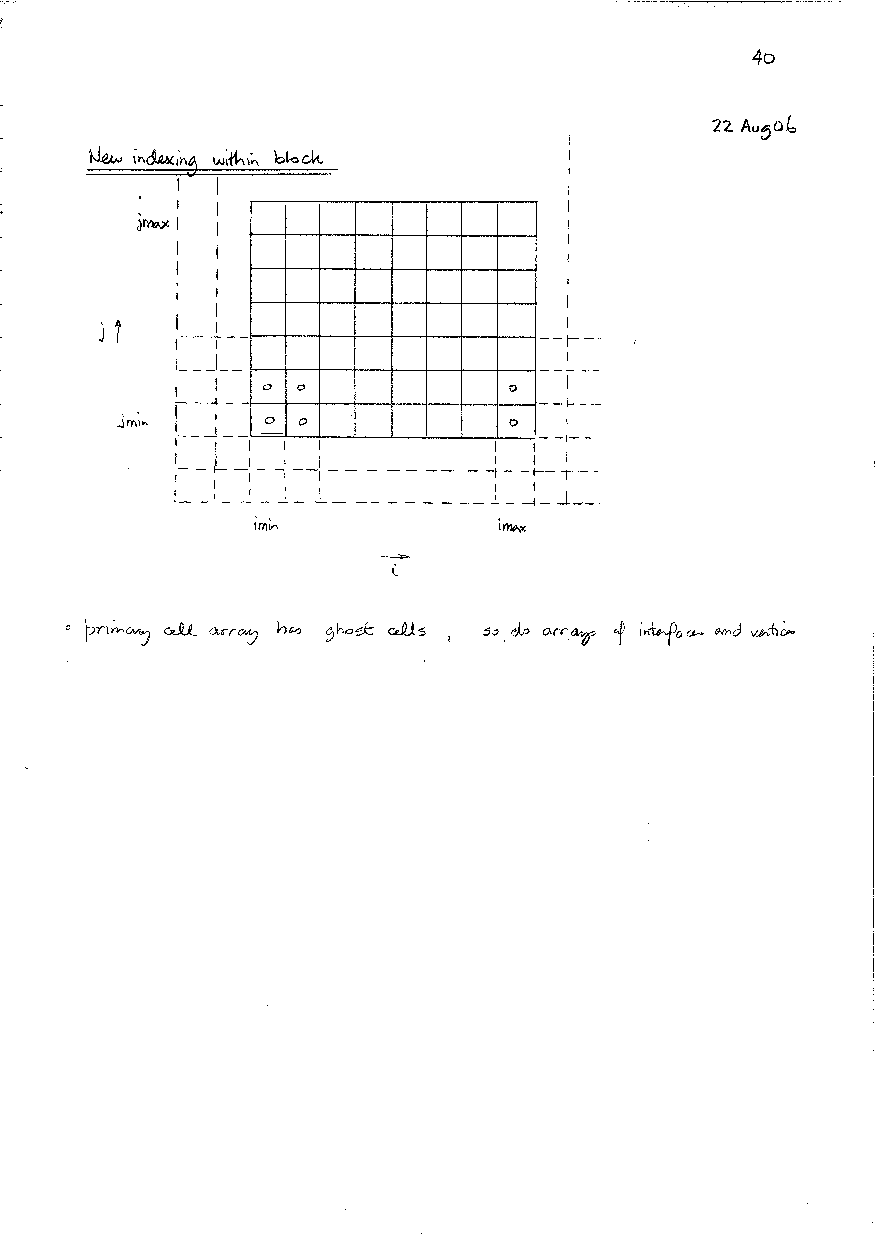
\includegraphics[width=10cm,viewport=48 316 295 509,clip=true]{figures/mbcns2-indexing-within-block.pdf} }
   \caption{Active and ghost cells for a single 2D block grid for \texttt{Eilmer3}.}
   \label{mbcns2-block-fig}
\end{figure}

\medskip
For a boundary common to two blocks, the ghost cells in the
buffer region of each block overlap the active cells of the adjacent block.
The only interaction that occurs between blocks is the 
exchange of boundary data, prior to the reconstruction phase of each time step.
For the \textit{shared memory} version of the code, 
the exchange of cell-average data along the block boundaries takes place as
a direct copy from the active-cell of one block to the ghost-cell of the other block.
Thus, the cells along the common boundary of each block must match in both number and position.
Some logic is used within the exchange routines to set the appropriate indexing direction for each boundary.
The information on the connections between block boundaries is stored in a (global) connectivity array.
For each boundary on each block, this array stores the
identity of the adjacent block and the name of the connecting boundary on the adjacent block.

\medskip
Except for this block-to-block communication (and the occasional checking of time step magnitudes),
the rest of the calculation can be done independently for all blocks.
Thus, the algorithm is fairly easy to implement on a multiple-instruction, multiple-data (MIMD) parallel computer and
we have a single-program-multiple-data (SPMD) version of the code 
for computationally-intensive facility calculations.
When running such simulations, there are many copies of the program running independently 
on separate processors, with each copy of the program handling the computation for a single block.
To exchange block-boundary data, each program instance must communicate with the other programs for adjacent blocks.
The communication and synchronisation tasks 
are handled via a standard message passing library, MPI~\cite{gropp_etal_1994a}. 

\subsection{Boundary Conditions}
%
The inviscid-component of applied boundary conditions is implemented by also filling in 
the ghost-cell data and then applying the normal reconstruction and flux calculation without
further discrimination of the boundary cells.
This approach covers solid/slip walls, inflow and outflow boundaries.

\medskip
For viscous simulations, boundaries may also be assigned as fixed temperature, 
no-slip or catalytic (chemical equilibrium at wall gas state) boundary conditions.
Such viscous boundary conditions also use data specified at the cell interfaces
that lie along the boundary surface.
These data are used in the derivative calculations that subsequently feed into 
the viscous fluxes.

\begin{figure}
   \centerline{ 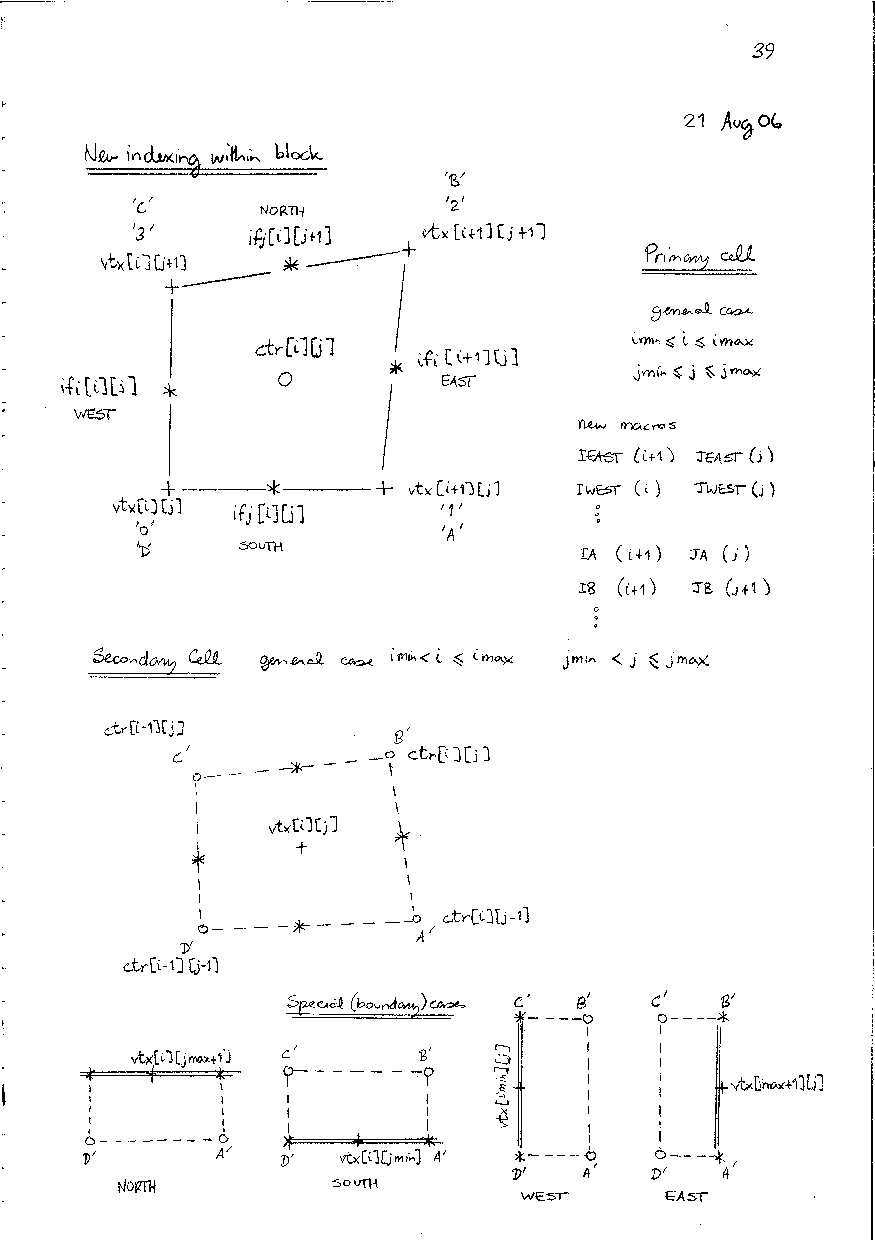
\includegraphics[width=120mm,viewport=28 16 396 515,clip=true]{figures/mbcns2-cell-and-interface-indexing.pdf} }
   \caption{Cell, interface and vertex indexing in 2D for \texttt{Eilmer3}.  The upper half of the figure
       shows the primary cells defining the finite-volumes for the conservation equations.
       The lower part of the figure shows the secondary cells, used for computing spatial derivatives.}
   \label{mbcns2-cell-fig}
\end{figure}

\medskip
There are also boundary conditions that allow the user to specify the ghost-cell data and boundary
interface data via user-written functions (via an embedded Lua interpreter).
These functions may also be used to bypass the internal flux calculators and specify the boundary
fluxes directly.
When exploring specialized boundary conditions, 
such as the mixing-plane interface for turbomachinery calculations,
the user can first implement them as Lua functions.


\subsection{Inviscid Flux Calculation}
%
The flow-states at the cell interfaces are calculated using a piecewise-parabolic scheme.
Before computing the inviscid fluxes at each interface, 
the velocity field is rotated into a local $(n,p,q)$-coordinate system
with unit vectors
%
\begin{eqnarray}
   \hat{n} & = & n_x ~ \hat{i} + n_y ~ \hat{j} + n_z ~ \hat{k} ~~~, \nonumber \\
   \hat{p} & = & p_x ~ \hat{i} + p_y ~ \hat{j} + p_z ~ \hat{k} ~~~, \nonumber \\
   \hat{q} & = & q_x ~ \hat{i} + q_y ~ \hat{j} + q_z ~ \hat{k} ~~~,
\end{eqnarray}
%
where $\hat{n}$ is normal and $\hat{p}, \hat{q}$ are tangental to the cell interface.
The normal and tangential velocity components
%
\begin{eqnarray}
   u_n & = & n_x ~ u_x + n_y ~ u_y + n_z ~ u_z ~~~, \nonumber \\
   u_p & = & p_x ~ u_x + p_y ~ u_y + p_z ~ u_z ~~~, \nonumber \\
   u_q & = & q_x ~ u_x + q_y ~ u_y + q_z ~ u_z ~~~,
\end{eqnarray}
%
are then used, together with the other flow properties either side of the interface, 
to compute the inviscid fluxes
%
\begin{equation}
\label{local-flux-vector-eqn}
   \left[
   \begin{array}{l}
      F_{mass} \\
      F_{n-momentum} \\
      F_{p-momentum} \\
      F_{q-momentum} \\
      F_{energy} \\
      F_{species-s}
   \end{array}
   \right]
   =
   \left[
   \begin{array}{l}
      \rho u_n \\
      \rho u_n u_n + p \\
      \rho u_n u_p \\
      \rho u_n u_q \\
      \rho u_n E + p u_n \\
      \rho u_n f_s
   \end{array}
   \right] ~~~,
\end{equation}
%
in the local reference frame.
These are then transformed back to the $(x,y,z)$ coordinate system as
%
\begin{equation}
   \overline{F} \cdot \hat{n} =
   \left[
   \begin{array}{l}
      F_{mass} \\
      F_{x-momentum} \\
      F_{y-momentum} \\
      F_{z-momentum} \\
      F_{energy} \\
      F_{species-s}
   \end{array}
   \right]
   =
   \left[
   \begin{array}{l}
      F_{mass} \\
      F_{n-momentum} n_x + F_{p-momentum} p_x + F_{q-momentum} q_x \\
      F_{n-momentum} n_y + F_{p-momentum} p_y + F_{q-momentum} q_y \\
      F_{n-momentum} n_z + F_{p-momentum} p_z + F_{q-momentum} q_z \\
      F_{energy} \\
      F_{species-s}
   \end{array}
   \right] ~~~.
\end{equation}

\medskip
For the simulation of shock and expansion tubes, the shock waves can be extremely strong
so we use the default adaptive scheme in which the equilibrium flux method (EFM)~\cite{macrossan_89} 
is applied near shocks and a modified AUSMDV calculator~\cite{wada_liou_94a} is applied elsewhere.

\subsubsection{Reconstruction}
%
The primary data held by the code are cell-average data, associated with cell centres.
To get the fluxes at cell interfaces, a variable-by-variable reconstruction is made of the flow field.
This is done in a one-dimensional fashion, working along one-index direction at a time.
\textit{Left} and \textit{Right} values ($w_L$ and $w_R$ respectively) of a flow variable at a cell interface
are evaluated as the corresponding cell average value plus a limited higher-order interpolated increment.
Given an array of cell-centres $[L1,L0,R0,R1]$ with an interface located between $L0$ and $R0$, the interpolated
values are
\begin{eqnarray}
  % PJ's mbcns workbook page 36 July, August 2006
  w_L & = & w_{L0} + \alpha_{L0} \left[ \Delta_{L+} \times \left( 2 h_{L0} + h_{L1} \right) + \Delta_{L-} \times h_{R0} \right] s_L ~~, \nonumber \\
  w_R & = & w_{R0} - \alpha_{R0} \left[ \Delta_{R+} \times h_{L0} + \Delta_{R-} \times \left( 2 h_{R0} + h_{R1} \right) \right] s_R ~~, \nonumber \\
  \Delta_{L-} & = & \frac{w_{L0} - w_{L1}}{\frac{1}{2} \left( h_{L0} + h_{L1}\right)} ~~, \nonumber \\
  \Delta_{L+} & = & \frac{w_{R0} - w_{L0}}{\frac{1}{2} \left( h_{R0} + h_{L0} \right)} ~ = ~ \Delta_{R-} ~~, \nonumber \\
  \Delta_{R+} & = & \frac{w_{R1} - w{R0}}{\frac{1}{2} \left( h_{R0} + h_{R1} \right)} ~~, \nonumber \\
  \alpha_{L0}  & = & \frac{h_{L0} / 2}{h_{L1} + 2 h_{L0} + h_{L0}} ~~, \nonumber \\
  \alpha_{R0}  & = & \frac{h_{R0} / 2}{h_{L0} + 2 h_{R0} + h_{R1}} ~~,
\end{eqnarray}
where the $h$ represents the width of a cell and the van Albada limiter\,\cite{vanalbada_etal_81} is implemented as
\begin{eqnarray}
 s_L & = & \frac{\Delta_{L-} \Delta_{L+} + |\Delta_{L-} \Delta_{L+}|}{\Delta_{L-}^2 + \Delta_{L+}^2 + \epsilon} ~~, \nonumber \\
 s_R & = & \frac{\Delta_{R-} \Delta_{R+} + |\Delta_{R-} \Delta_{R+}|}{\Delta_{R-}^2 + \Delta_{R+}^2 + \epsilon} ~~, \nonumber \\
 \epsilon & = & 1.0 \times 10^{-12} ~~. \nonumber
\end{eqnarray}
Finally, minimum and maximum limits are applied so that the newly interpolated values 
lie within the range of the original cell-centred values. 
Unlimited, this reconstruction scheme has third-order truncation errors and, with the limiter active, a sine function
is reconstructed with an effective truncation error order of 2.7.
 
\medskip
Typically, reconstruction is done for density, internal energy, velocity components, and species mass fractions.
Other flow quantities that are needed at the interfaces for the inviscid flux calculation 
are then obtained from the thermochemical model.

\subsubsection{EFM Calculation}
% We write the LaTeX just as the code is written in efm.cxx.
\newcommand{\dtwspi}{\frac{1}{2 \sqrt{\pi}}}
\newcommand{\rtL}{R T_L}
\newcommand{\rtR}{R T_R}
\newcommand{\conpjp}{\frac{1}{2} \frac{\gamma + 1}{\gamma - 1}}
\newcommand{\cmpL}{\sqrt{2 R T_L}}
\newcommand{\cmpR}{\sqrt{2 R T_R}}
\newcommand{\snL}{\frac{u_{nL}}{\cmpL}}
\newcommand{\snR}{\frac{u_{nR}}{\cmpR}}
\newcommand{\hvsqL}{\frac{1}{2}\left(u_{nL}^2 + u_{pL}^2\right)}
\newcommand{\hvsqR}{\frac{1}{2}\left(u_{nR}^2 + u_{pR}^2\right)}
\newcommand{\hL}{e_L + \frac{p_L}{\rho_L}}
\newcommand{\hR}{e_R + \frac{p_R}{\rho_R}}
%
The equilibrium flux method (EFM)~\cite{macrossan_89} is used for its dissipative nature in the
vicinity of very strong compressions. 
The method assumes that the gas is in equilibrium and the molecular velocities of the gas
either side of the interface can be described with the Boltzmann distribution. 
As implemented in Reference~\cite{petrie_repar_1997a}, 
the flux of mass from the left state, moving to the right is
\begin{equation}
 F_{massL} = W_L^+ ~ \rho_L ~ u_{nL} + D_L^+ ~ \rho_L ~ \cmpL ~~,
\end{equation}
where
\begin{eqnarray}
 W_L^+ & = & \frac{1}{2} \left( 1 + {\rm erf}\left(\frac{u_{nL}}{\cmpL} \right) \right) ~~, \nonumber \\
 D_L^+ & = & \dtwspi {\rm exp}\left( -\left( \frac{u_{nL}}{\cmpL} \right)^2 \right) ~~, \nonumber \\
 {\rm erf}(s) & = & \frac{2}{\sqrt{\pi}} \int_0^s \exp(-t^2) \,dt.
\end{eqnarray}
Similarly, the flux of mass from the right state, moving to the left is
\begin{equation}
 F_{massR} = W_R^- ~ \rho_R ~ u_{nR} + D_R^- ~ \rho_R ~ \cmpR ~~,
\end{equation}
where
\begin{eqnarray}
 W_R^- & = & \frac{1}{2} \left( 1 - {\rm erf}\left(\frac{u_{nR}}{\cmpR} \right) \right) ~~, \nonumber \\
 D_R^- & = & \dtwspi {\rm exp}\left( -\left( \frac{u_{nR}}{\cmpR} \right)^2 \right) ~~.
\end{eqnarray}
The flux vector components are then
\begin{eqnarray}
 F_{mass} & = & F_{massL} + F_{massR} ~~, \nonumber \\
 F_{n-momentum} & = & F_{massL} ~ u_{nL} + F_{massR} ~ u_{nR} + W_L^+ ~ p_L + W_R^- ~ p_R ~~, \nonumber \\
 F_{p-momentum} & = & F_{massL} ~ u_{pL} + F_{massR} ~ u_{pR} ~~, \nonumber \\
 F_{energy} & = & \left( W_L^+ ~ \rho_L ~ u_{nL} \right) \left( \hL + \hvsqL \right) \nonumber \\
            &   & + \left( W_R^- ~ \rho_R ~ u_{nR} \right) \left( \hR + \hvsqR \right) \nonumber \\
            &   & + \left( D_L^+ ~ \cmpL ~ \rho_L \right) \left( \hvsqL + \conpjp \rtL \right) \nonumber \\
            &   & + \left( D_R^- ~ \cmpR ~ \rho_R \right) \left( \hvsqR + \conpjp \rtR \right)~~.
\end{eqnarray}
Species mass fractions are just transported by the net mass flux as scalar quantities.
Note that the gas constants, $R$ and $\gamma$, are not really constant; 
they are density-weighted averages derived from the local values for left and right gas states.
 
\subsubsection{AUSMDV calculation}
%
\newcommand{\ruhalf}{(\rho u)_\frac{1}{2}}
\newcommand{\rusq}{(\rho u^2)}
%
Most of the flow field fluxes are computed with the AUSMDV~\cite{wada_liou_94a} 
because of its reasonably low dissipation.
The calculation procedure starts by computing the weighting parameters for the velocity splitting
\begin{eqnarray}
  \alpha_L & = & \frac{2 ~ p_L / \rho_L}{p_L / \rho_L + p_R / \rho_R} ~~, \nonumber \\
  \alpha_R & = & \frac{2 ~ p_R / \rho_R}{p_L / \rho_L + p_R / \rho_R} ~~, 
\end{eqnarray}
and the sound speed and Mach numbers in the normal direction to the interface
\begin{eqnarray}
  a_m & = & \max(a_L, a_R) ~~, \nonumber \\
  M_L & = & \frac{u_{nL}}{a_m} ~~, \nonumber \\
  M_R & = & \frac{u_{nR}}{a_m} ~~.
\end{eqnarray}
The components from pressure splitting are then
\begin{eqnarray}
 p_L^+ & = & \frac{p_L}{4} ( M_L + 1 )^2 ~(2 - M_L) ~~, ~~ |M_L| \le 1.0 ~~, \nonumber \\
       & = & \frac{p_L ~ du_L}{u_{nL}} ~~, ~~ {\rm otherwise} ~~, \nonumber \\  
 p_R^- & = & \frac{p_R}{4} ( M_R - 1 )^2 ~(2 + M_R) ~~, ~~ |M_R| \le 1.0 ~~, \nonumber \\
       & = & \frac{p_R ~ du_R}{u_{nR}} ~~, ~~ {\rm otherwise} ~~,  
\end{eqnarray}
where $du_L = \frac{( u_{nL} + |u_{nL}|)}{2} $ and $du_R = \frac{(u_{nR} - |u_{nR}|)}{2}$.
The components from the velocity splitting are
\begin{eqnarray}
 u_L^+ & = & \alpha_L \left( \frac{( u_{nL} + a_m )^2}{4 ~ a_m} - du_L \right) + du_L  ~~, ~~ |M_L| \le 1.0 ~~, \nonumber \\
       & = & du_L ~~, ~~ {\rm otherwise} ~~, \nonumber \\  
 u_R^- & = & - \alpha_R \left( \frac{( u_{nR} - a_m )^2}{4 ~ a_m} + du_R \right) + du_R  ~~, ~~ |M_R| \le 1.0 ~~, \nonumber \\
       & = & du_R ~~, ~~ {\rm otherwise} ~~,  
\end{eqnarray}
These components are then combined into a mass flux
\begin{equation}
 \ruhalf = u_L^+ ~ \rho_L + u_R^- ~ \rho_R
\end{equation}
and a pressure flux
\begin{equation}
 p_\frac{1}{2} =  p_L^+ + p_R^-  
\end{equation}
and a normal-momentum flux $(\rho u^2)_\frac{1}{2}$ as a blend of AUSMV and AUSMD fluxes
\begin{eqnarray}
  \rusq_{AUSMV} & = & u_L^+ ~ \rho_L ~ u_{nL} + u_R^- ~ \rho_R ~ u_{nR}~~, \nonumber \\
  \rusq_{AUSMD} & = & \frac{1}{2} \left( \ruhalf (u_{nL} + u_{nR}) - |\ruhalf| (u_{nR} - u_{nL}) \right)~~, \nonumber \\
  \rusq_\frac{1}{2} & = & (\frac{1}{2} + s) \rusq_{AUSMV} + (\frac{1}{2} - s) \rusq_{AUSMD} ~~,
\end{eqnarray}
with the switching function, $s$,  based on the pressure gradient
\begin{equation}
  s = \frac{1}{2} \min \left( 1, K \frac{|p_R - p_L|}{\min(p_L, p_R)} \right) ~~,
\end{equation}
with $K = 10$.

\medskip
The flux vector components can be assembled from these pieces as
\begin{eqnarray}
 F_{mass} & = & \ruhalf ~~, \nonumber \\
 F_{n-momentum} & = & \rusq_\frac{1}{2} + p_\frac{1}{2} ~~,
\end{eqnarray}
and depending on which way the wind is blowing, 
the remaining flux vector components are assembled from either the right or left flow properties.
For $\ruhalf \ge 0$, 
\begin{eqnarray}
 F_{p-momentum} & = & \ruhalf ~ u_{pL} ~~, \nonumber \\
 F_{energy} & = & \ruhalf ~ H_L ~~. \\
\end{eqnarray}
otherwise
\begin{eqnarray}
 F_{p-momentum} & = & \ruhalf ~ u_{pR} ~~, \nonumber \\
 F_{energy} & = & \ruhalf ~ H_R ~~. \\
\end{eqnarray}
where $H = e + \frac{p}{\rho} + \frac{1}{2} \left( u_{n}^2 + u_{p}^2 \right)$ is the total enthalpy
of the gas.
Again, species mass fractions are just transported by the mass flux as scalar quantities.

\medskip
Finally, an entropy fix is applied, as per Section 3.5 in Reference~\cite{wada_liou_94a}.
This first determines if the interface includes an expansion sonic point\\
\begin{center}
 Case A: $u_{nL} - a_L < 0$ and $u_{nR} - a_R > 0$\\
 Case B: $u_{nL} + a_L < 0$ and $u_{nR} + a_R > 0$
\end{center}
and increments the flux if only a single expansion wave is detected
\newcommand{\dua}{\Delta_{ua}}
\begin{eqnarray}
 F_{mass} & -= & \dua ~ (\rho_R - \rho_L) ~~, \nonumber \\
 F_{n-momentum} & -= & \dua ~ (\rho_R u_{nR} - \rho_L u_{nL})~~, \nonumber \\
 F_{p-momentum} & -= & \dua ~ (\rho_R u_{pR} - \rho_L u_{pL})~~, \nonumber \\
 F_{energy} & -= & \dua ~ (\rho_R H_R - \rho_L H_L)~~,
\end{eqnarray}
where
\begin{eqnarray}
 \dua & = & 0.125 ((u_{nR} - a_R) - (u_{nL} - a_L)) ~,{\rm ~ for~ A~ and~ not~ B}, \nonumber \\
      & = & 0.125 ((u_{nR} + a_R) - (u_{nL} + a_L)) ~,{\rm ~ for~ B~ and~ not~ A}, \nonumber \\
      & = & 0~, {\rm ~ otherwise}.
\end{eqnarray}


\subsubsection{Shock Detector}
%
The switching between the two flux calculators is governed by a shock (or compression) detector.
This is simply a measure of the relative change in normal velocity at interfaces.
Specifically, we indicate a strong compression at cell-interface $i + \frac{1}{2}$ when
\begin{equation}
   \frac{u_{n,i+1} - u_{n,i}}{\min(a_{i+1}, a_i)} < \rm Tol ~~,
\end{equation}
where Tol is the compression tolerance and is typically set at -0.05.
This measure is applied to all interfaces in a block and then a second pass propagates the information 
to near-by interfaces.
If a first cell-interface is identified as having a strong compression, the EFM flux calculator is used 
for all interfaces attached to the cell containing that first cell-interface. 


\subsection{Viscous Fluxes}
%
The viscous flux calculation is then performed based on the the updated cell-centre flow state.
The spatial derivatives required in the viscous stress and heat flux terms, Eq.~\ref{eq:taus} and~\ref{eq:qs}, 
are evaluated as
\begin{equation}
 \nabla \phi = \frac{1}{V} \oint_S \phi \, \hat{n} \, dA \text{,}
 \label{eq:divergence-theorem}
\end{equation}
where $\phi$ a scalar quantity and the surface $S$ defines the secondary cell surrounding a primary-cell vertex, 
as shown in Figure~\ref{mbcns2-cell-fig}.
When used in the viscous fluxes, the vertex values are averaged to obtain a midface value.
All evaluations are done within a block and
secondary cells of half size are used along the boundary faces of the block.
Viscous boundary conditions for velocity (\textit{e.g.} no slip) and temperature are 
applied by using data that was specified at cell interfaces along the boundary.
In 3D, further special cases for the derivatives are encountered for the edges of the block, 
which are evaluated with a least squares fit of the function $\phi = a\, x + b\, y + c\, z + d$,
and for corners where there is just enough data to fit the same linear function.
In 2D, a line integral corresponding to Eq.(\ref{eq:divergence-theorem}) is done, just within the (x,y)-plane.
Also in 2D, only the corners need to be treated by fitting a bilinear function. 

